% ********** Rozdział 4 **********
\chapter{Prezentacja warstwy użytkowej projektu}

\section{Opis interfejsu użytkownika}

\begin{figure}[htbp]
  \centering
  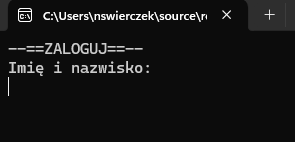
\includegraphics[width=0.6\textwidth]{zalog.png}
  \caption{Panel logowania}
  \label{fig:zalog}
\end{figure}

\begin{figure}[htbp]
  \centering
  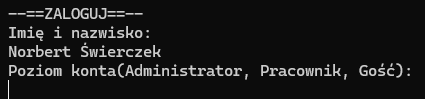
\includegraphics[width=0.6\textwidth]{zalog2.png}
  \caption{Wybór poziomu konta}
  \label{fig:zalog2}
\end{figure}

\begin{figure}[htbp]
  \centering
  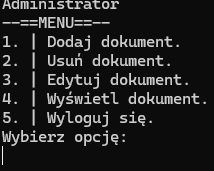
\includegraphics[width=0.6\textwidth]{menu.png}
  \caption{Główne menu systemu z opcjami CRUD (tworzenie, edycja, usuwanie, przeglądanie dokumentów) oraz możliwością wylogowania}
  \label{fig:menu}
\end{figure}

\begin{figure}[htbp]
  \centering
  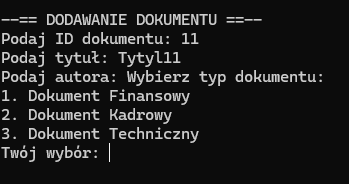
\includegraphics[width=0.7\textwidth]{dodawanie.png}
  \caption{Proces dodawania nowego dokumentu z wyborem typu (Finansowy/Kadrowy/Techniczny) i specjalnym polem kwoty dla dokumentów finansowych}
  \label{fig:dodawanie}
\end{figure}

\begin{figure}[htbp]
  \centering
  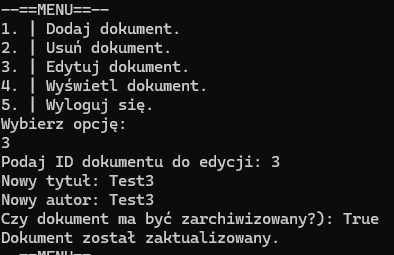
\includegraphics[width=0.7\textwidth]{edytuj.png}
  \caption{Edycja istniejącego dokumentu z możliwością zmiany tytułu, autora oraz statusu archiwizacji}
  \label{fig:edycja}
\end{figure}

\begin{figure}[htbp]
  \centering
  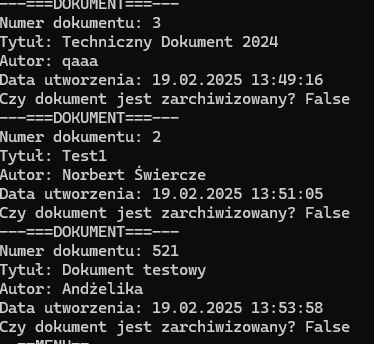
\includegraphics[width=0.8\textwidth]{wyswietl.png}
  \caption{Przeglądanie dokumentów ze szczegółowymi informacjami: ID, tytuł, autor, data utworzenia i status archiwizacji}
  \label{fig:przegladanie}
\end{figure}

\begin{figure}[htbp]
  \centering
  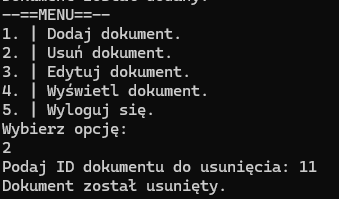
\includegraphics[width=0.6\textwidth]{usun.png}
  \caption{Mechanizm usuwania dokumentów po podaniu identyfikatora z potwierdzeniem operacji}
  \label{fig:usuwanie}
\end{figure}


% ********** Koniec rozdziału **********
